\documentclass{article}
\usepackage{inputenc, graphicx, circuitikz, mathtools}

\title{On-Site Homework 8\\
  E 2420}
  \author{\boxed{\text{Patrick Harrington}}}

  \begin{document}
  \maketitle

  \section{Tuning the VCO}

  \begin{figure}[h!]
    \centering
    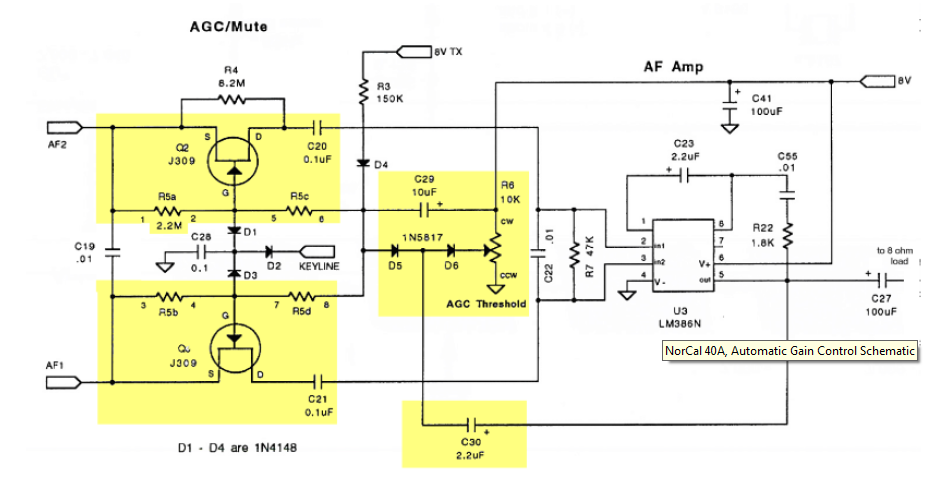
\includegraphics[scale=0.6]{AGC.png}
    \label{AGC}
    \caption{AGC schematic}
  \end{figure}
  The following steps were taken in order to tune the
  VCO:

  \begin{enumerate}
    \item   Install a 3k$\Omega$ resistor in the
      $C_{19}$ holes.
    \item   The function generator was
      attached to the antenna input, with a
      100 $mV_{pp}$ at 7.02 MHz.
    \item   The beat frequency
      oscillator was set to its
      maximum value by tuning the
      variable capacitor $C_{17}$.
    \item   The input RF
      frequency was tuned to
      produce a maximum signal
      to the input of the audio
      mixer/product detector. 
    \item   This process
      was repeated at the
      output of each
      crystal.
    \item   The RF
      mixer
      potentiometer
      was set to
      the middle of
      its setting.
    \item
      The
      oscilloscope
      probe
      was
      placed
      at the
      3
      k$\Omega$
      resistor
      (with
      one end
      still
      connected
      to
      ground).
      The
      audio
      signal
      was
      kept
      under
      500
      mVpp.
    \item
      The
      potentiometer
      was
      varied
      for
      the
      VCO
      until
      an
      audio
      signal
      was
      observed.
  \end{enumerate}

  \subsection{Range
    of
    Audio
  Frequencies}
  The
  range
  of
  audio
  frequencies
  that
  was
  obtained
  by
  changing
  the
  VCO
  was
  $\boxed{385Hz-1.16kHz}$:

  \section{Building
    the
    Automatic
    Gain
    Controller
  (AGC)}
  The
  highlighted
  parts
  in
  Figure~\ref{AGC}
  were
  soldered:
  \subsection{Measuring
    Range
    of
    Control
  Voltages}
  A
  multimeter
  was
  used
  to
  measure
  the
  DC
  voltage
  at
  the
  anode
  of
  $D_5$.
  For
  AC
  measurements,
  measurements
  were
  taken
  at
  the
  8$\Omega$
  resistor.
  Starting
  with
  1$V_{RMS}$,measurements
  were
  taken
  of
  the
  DC
  and
  AC
  (Audio)
  output
  voltages,
  and
  is
  plotted
  in
  Figure~\ref{controlvolts}.

  \begin{figure}[ht!]
    \centering
    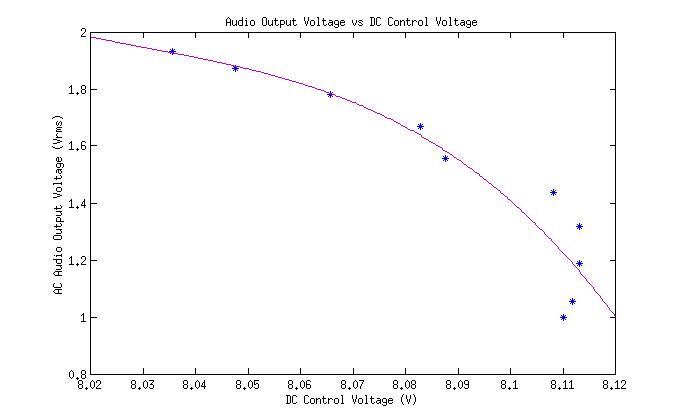
\includegraphics[scale=0.5]{controlvolts.jpg}
    \label{controlvolts}
    \caption{Plot
      of
      DV
      Control
      Voltages
      against
      AC
      Audio
      Output
    Voltages}
  \end{figure}

  \subsection{Measuring
    AGC
    Output
    on
    Audio
  Voltage}
  The
  AGC
  capacitor
  was
  $C_{29}$
  was
  then
  installed
  followed
  by
  $C_{30}$,
  the
  coupling
  capacitor.
  The
  effect
  of
  the
  AGC
  on
  the
  output
  voltage
  was
  measured,
  and
  is
  plotted
  in
  Figure~\ref{AGCplot}.

  \begin{figure}[ht!]
    \centering
    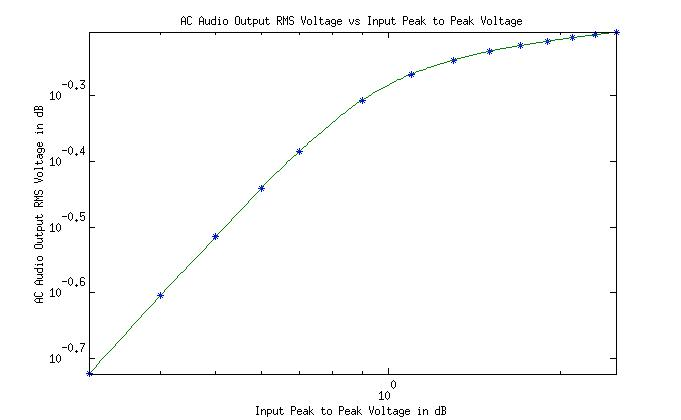
\includegraphics[scale=0.5]{AGCplot.jpg}
    \label{AGCplot}
                                                                                                                    %Log-Log
                                                                                                                    %plot%
    \caption{Effect
      of
      the
      AGC
      on
      the
      output
      audio
      voltage.
      The
      AGC
      kicks
      in
      at
      about
    1.}
  \end{figure}

  The
  slope
  of
  the
  line
  before
  the
  AGC
  kicks
  in
  was
  found
  to
  be
  roughly
  $\boxed{0.563}$
  and
  the
  slope
  of
  the
  line
  after
  the
  AGC
  kicks
  in
  was
  found
  to
  be
  roughly
  $\boxed{0.067}$.
  Since
  the
  units
  are
  $\frac{Volts
    \cdot
  dB}{Volts
    \cdot
  dB}$,
  there
  are
  no
  units
  for
  the
  slope.

  \end{document}
